\documentclass[xcolor=table,10pt,final]{beamer}
\renewcommand\mathfamilydefault{\rmdefault}

\setbeamertemplate{navigation symbols}{}
\usepackage{amsmath,amsfonts,amssymb,pxfonts,xspace}
\usepackage{textcomp}
\usepackage{lmodern}
\usepackage{verbatim}
\usepackage{graphicx}
\usepackage{listings}
\usepackage[T1]{fontenc}

%\def \audience {}

\lstset{
    language=Python,
    basicstyle=\footnotesize,
    keywordstyle=\color[rgb]{0.1,0.8,0.1}\bfseries,
    commentstyle=\color{blue},
    numbers=left,
    stringstyle=\ttfamily\color{red!50!brown},
    showstringspaces=false}
\lstset{literate=%
   *{0}{{{\color{red!20!violet}0}}}1
    {1}{{{\color{red!20!violet}1}}}1
    {2}{{{\color{red!20!violet}2}}}1
    {3}{{{\color{red!20!violet}3}}}1
    {4}{{{\color{red!20!violet}4}}}1
    {5}{{{\color{red!20!violet}5}}}1
    {6}{{{\color{red!20!violet}6}}}1
    {7}{{{\color{red!20!violet}7}}}1
    {8}{{{\color{red!20!violet}8}}}1
    {9}{{{\color{red!20!violet}9}}}1
}

\begin{document}
\definecolor{navy}{RGB}{0,0,128}
\lstset{language=Python}

\title{Python for Scientific Computing}
\subtitle{Lecture 4: Code Optimization}
\author{{\bf Esteban Meneses}\\emeneses@pitt.edu\\{\em Center for Simulation and Modeling (SaM)}}
\date{\today}
\frame{\titlepage}

\ifx \audience \undefined
\begin{frame}
	\frametitle{This week in the Workshop}
	\begin{itemize}
		\item {\bf Monday} (Esteban)
		\begin{itemize} 
			\item Why is the code so slow?
			\item Algorithm design, profiler and performance tips
		\end{itemize}
		\item {\bf Wednesday} (Patrick)
		\begin{itemize} 
			\item Building scientific Python codes efficiently 
			\item NumPy and SciPy libraries
		\end{itemize}
		\item {\bf Friday} (Joshua)
		\begin{itemize} 
			\item Speeding up Python codes
			\item Cython
		\end{itemize}
	\end{itemize}
\end{frame}
\else
\fi

\begin{frame}
	\frametitle{What does \emph{Code Optimization} mean?}
			\begin{itemize}
				\item Accelerate your code
				\item Algorithm design
				\begin{itemize}
					\item Implementation alternatives
					\item Algorithmic alternatives
				\end{itemize}
				\item Profiler
				\item Performance recommendations
			\end{itemize}
\end{frame}

\begin{frame}
\hfill \emph{Premature optimization is the root of all evil}

\hfill Donald Knuth
\end{frame}

{\setbeamercolor{background canvas}{bg=navy}
\begin{frame}
	\frametitle{\textcolor{yellow}{Exercise 1}}
	\textcolor{white}{Write a Python function to compute the \emph{n-th Fibonacci} number.\newline\newline
	 {\tt fibonacci(0) = 0\\
	 fibonacci(1) = 1\\
	 fibonacci(n) = fibonacci(n-1) + fibonacci(n-2)}\newline\newline
	 Example: \\ {\tt > fibonacci(10)\\55}
	}
\end{frame}
}

\begin{frame}[fragile]
	\frametitle{Recursive Fibonacci Function}	
	\begin{lstlisting}[language=Python]
def fibonacci(n):
  if n = = 0:
    return 0
  elif n = = 1:
    return 1
  else:
    return fibonacci(n-1) + fibonacci(n-2)
	\end{lstlisting}
\end{frame}

\ifx \audience \undefined
\begin{frame}
	\frametitle{Recursion in Hollywood}
	\begin{columns}[t,totalwidth=\textwidth]
		\begin{column}{.7\linewidth}
			\\
			\vspace{-2.0cm}
			
\includegraphics[scale=0.12]{inception}
		\end{column}
		\begin{column}{.3\linewidth}
			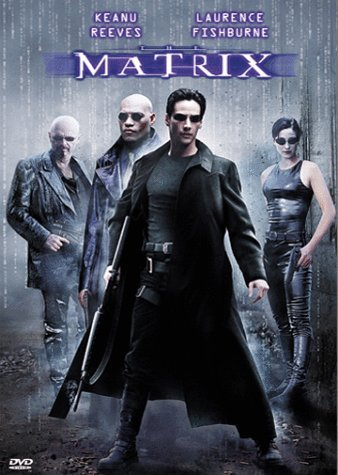
\includegraphics[scale=0.2]{matrix}\\ \vspace{0.5cm}
			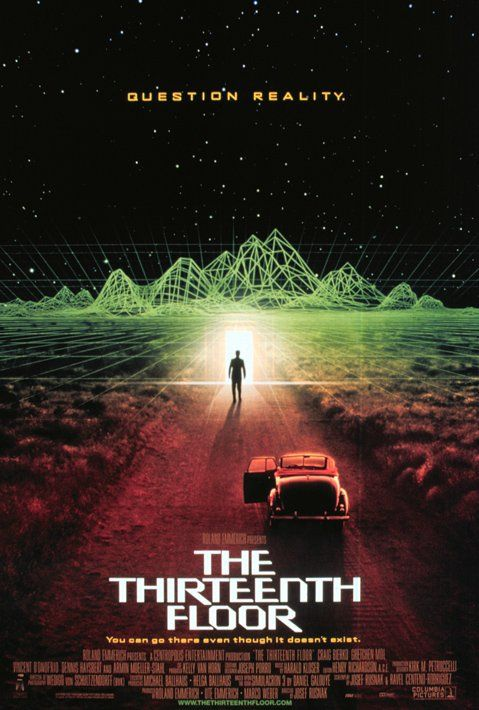
\includegraphics[scale=0.14]{floor}			
		\end{column}
	\end{columns}
\end{frame}
\else
\fi

\begin{frame}
	\frametitle{What is recursion?}
	\begin{itemize}
		\item Mechanism to solve problems through recursive functions
		\item A recursive function calls itself (directly or indirectly) with a different set of parameters
		\item Matches the mathematical description of many processes
		\item Recursive solutions are usually concise
		\item Each recursive call requires a new context to be created
		\item Typical in functional programming languages (Lisp)
	\end{itemize}
\end{frame}

\begin{frame}
	\frametitle{What is iteration?}
	\begin{itemize}
		\item Mechanism to solve problems through repetition of operations (loops)
		\item Handles the dependence between values across iterations naturally
		\item Scientific algorithms tend to be iterative in nature
		\item No new context is necessary for each iteration
		\item Typical in imperative programming languages (Fortran, C)
	\end{itemize}
\end{frame}

\begin{frame}[fragile]
	\frametitle{Iterative Fibonacci function}
	\begin{lstlisting}[language=Python]
def fibonacci_iter(n):
  fn_2 = 0
  fn_1 = 1
  for i in xrange(1,n):
    fn = fn_1 + fn_2
    fn_2 = fn_1
    fn_1 = fn
  return fn
	\end{lstlisting}
\end{frame}

\begin{frame}
	\frametitle{Recursion vs Iteration}
	\begin{itemize}
		\item Recursion is usually more elegant (clear, concise)
		\begin{itemize}
			\item Functional solutions express \emph{what} to compute
		\end{itemize}
		\item Iteration is generally more efficient
		\begin{itemize}
			\item Imperative solutions express \emph{what} and \emph{how} to compute
		\end{itemize}
		\item Tradeoff between elegance and performance
		\item Recursion and iteration are theoretically equivalent 
	\end{itemize}
\end{frame}

\begin{frame}
	\frametitle{Python Profiler}
	\begin{itemize}
		\item Provides a performance description of a program
		\item Magic functions in IPython
		\begin{itemize}
			\item Special commands to modify execution or environment
			\item Examples: \%edit, \%run, \%env
			\item Get timing information: \%time, \%timeit 
			\item Get profile information: \%prun 
		\end{itemize}
		\item Line profiler
		\begin{itemize}
			\item Install {\tt line\_profiler} and {\tt kernprof} modules
		\end{itemize}
	\end{itemize}
\end{frame}

{\setbeamercolor{background canvas}{bg=navy}
\begin{frame}
	\frametitle{\textcolor{yellow}{Exercise 2}}
	\textcolor{white}{Write a Python function to sort a list of integers in increasing order using the \emph{bubble sort} algorithm.\newline\newline
	{\tt The bubble sort algorithm sweeps a list of integers L swapping values L[i] and L[i+1] if L[i]>L[i+1]. It repeats this process until no elements are swapped.}\newline\newline
	Example: \\ {\tt > L = [9,8,7,6,5,4,3,2,1] }\\ {\tt > bubble\_sort(L)} \\ {\tt > L}\\ {\tt > [1,2,3,4,5,6,7,8,9]}
	}
\end{frame}
}

\begin{frame}[fragile]
	\frametitle{Bubble Sort Function}
	\begin{lstlisting}[language=Python]
def bubble_sort(list):
    """ Sorts a list using bubble sort algorithm """
    change = True
    while change:
        change = False
        for j in xrange(len(list)-1):
            if list[j] > list[j+1]:
                list[j],list[j+1] = list[j+1],list[j]
                change = True
	\end{lstlisting}
\end{frame}


\begin{frame}[fragile]
	\frametitle{Line Profile of Bubble Sort}
	{\tt ./kernprof.py -l -v profile.py} \newline \newline
	\centering 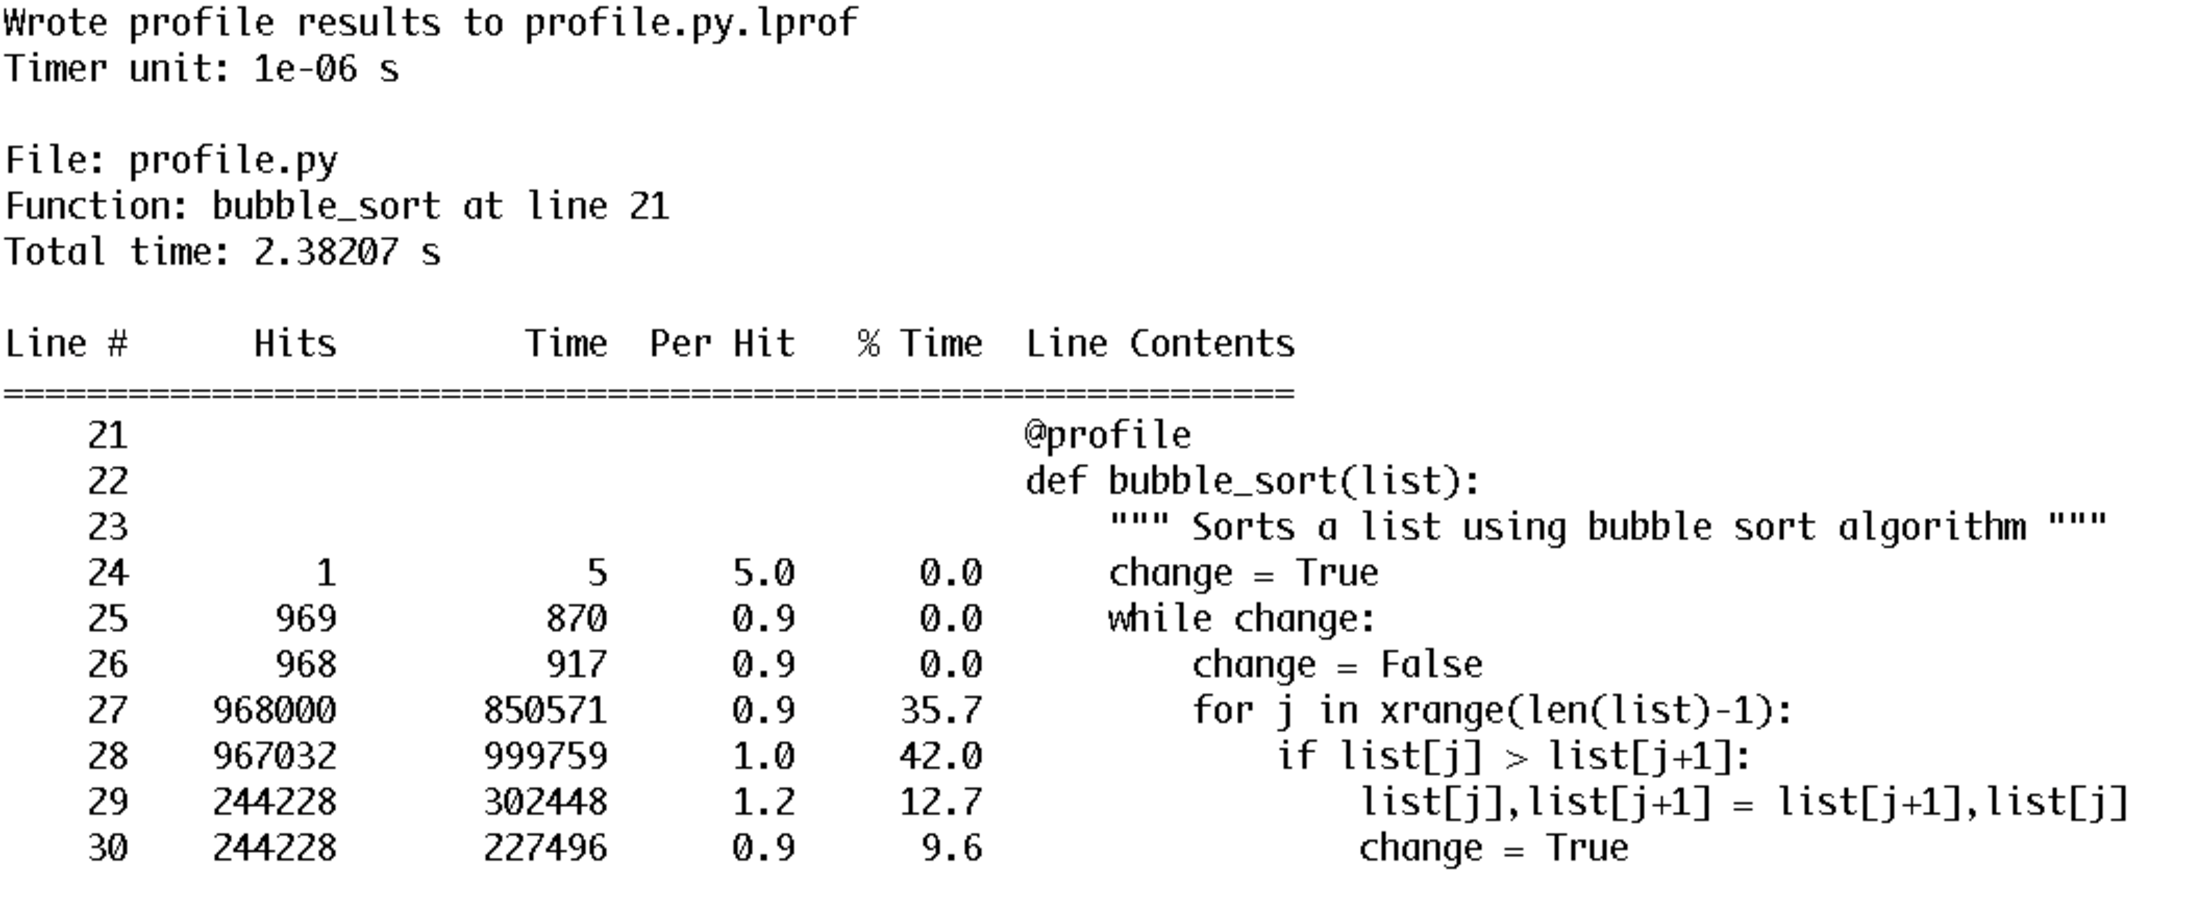
\includegraphics[scale=0.3]{profile}	
\end{frame}

\begin{frame}[fragile]
	\frametitle{Merge Sort Function}
	\begin{lstlisting}[language=Python]
def merge_sort(list):
    """ Sorts a list using merge sort algorithm """
    if len(list) == 1:
        return
    middle = len(list)/2
    left = list[0:middle]
    right = list[middle:len(list)]
    merge_sort(left)
    merge_sort(right)
    merge(left,right,list)
	\end{lstlisting}
\end{frame}

\begin{frame}[fragile]
	\frametitle{Merge Function}
	\begin{lstlisting}[language=Python]
def merge(left,right,list):
    """ Marges left and right sublists into list """
    left_max = len(left)-1
    right_max = len(right)-1
    left_index = 0
    right_index = 0
    for i in range(len(list)):
        if left_index > left_max:
            list[i] = right[right_index]
            right_index += 1
            continue
        if right_index > right_max:
            list[i] = left[left_index]
            left_index += 1
            continue
        if left[left_index] < right[right_index]:
            list[i] = left[left_index]
            left_index += 1
        else:
            list[i] = right[right_index]
            right_index += 1
	\end{lstlisting}
\end{frame}

\begin{frame}
	\frametitle{Algorithmic Complexity}
	\begin{itemize}
		\item A measure of how many operations are performed per input value
		\item Described as a function of $n$, the input size
		\item Big $O$ notation represents the worst-case scenario
		\item Sorting algorithms:
		\begin{itemize}
			\item Bubble sort: $O(n^2)$
			\item Merge sort: $O(n\log(n))$
		\end{itemize}
		\item The smaller the complexity function, the better scalability
		\item {\small $O(1)<O(\log(n))<O(n)<O(n\log(n))<O(n^2)<O(n^3)<O(e^n)$}
	\end{itemize}
\end{frame}

\begin{frame}[fragile]
	\frametitle{Iterators}
	\begin{itemize}
		\item Efficient in the use of memory
		\item On-demand object creation
		\item Example: {\tt range} vs {\tt xrange}
			\begin{lstlisting}[language=Python]
for x in range(10)
  foo(x)
			\end{lstlisting}
			\begin{lstlisting}[language=Python]
for x in xrange(10)
  foo(x)
			\end{lstlisting}
	\end{itemize}
\end{frame}

\begin{frame}[fragile]
	\frametitle{Map Function}
	\begin{itemize}
		\item Applies a function to each element of a list
		\item Works directly if each operation is independent
		\item Avoids overhead of {\tt for} loop
		\item Example:
			\begin{lstlisting}[language=Python]
final_list = []
for x in list:
    final_list.append(foo(x))
			\end{lstlisting}
			\begin{lstlisting}[language=Python]
final_list = map(foo,list)
			\end{lstlisting}
		\item List comprehension is a syntactic sugar of map
			\begin{lstlisting}[language=Python]
final_list = [foo(x) for x in list]
			\end{lstlisting}
	\end{itemize}
\end{frame}

\begin{frame}[fragile]
	\frametitle{Join Operation on Strings}
	\begin{itemize}
		\item Faster than loops to accumulate results in a list
		\item Avoids overhead of {\tt append} function
		\item Example:
			\begin{lstlisting}[language=Python]
s = ""
for x in list:
  s += foo(x)
			\end{lstlisting}
			\begin{lstlisting}[language=Python]
list_foo = [foo(item) for item in list]
s = "".join(list_foo)
			\end{lstlisting}
	\end{itemize}
\end{frame}


\begin{frame}[fragile]
	\frametitle{Local Variables}
	\begin{itemize}
		\item Faster to access than global variables
		\item Safer, more modular code
		\item Example:
			\begin{lstlisting}[language=Python]
sum = 0
def foo(n):
  global sum
  for x in xrange(n+1):
    sum += x
			\end{lstlisting}
			\begin{lstlisting}[language=Python]
sum = 0
def foo(n):
  sum = 0
  for x in xrange(n+1):
    sum += x
  return sum
sum += foo(n)
			\end{lstlisting}
	\end{itemize}
\end{frame}

\begin{frame}[fragile]
	\frametitle{Exceptions}
	\begin{itemize}
		\item Model abnormal behavior
		\item Disrupts the execution flow 
		\item Use {\tt raise} command to throw an exception
		\item Use {\tt try} and {\tt except} to handle an exception
		\item Example:
			\begin{lstlisting}[language=Python]
def foo(n):
  if n < 0:
    raise Exception("Negative Value")
try:
  foo(n)
except Exception:
  foo(-n)
			\end{lstlisting}
	\end{itemize}
\end{frame}

\begin{frame}[fragile]
	\frametitle{Exceptions (cont.)}
	\begin{itemize}
		\item Faster than conditional statements
		\item Example:
			\begin{lstlisting}[language=Python]
repetitions = {}
for word in words:
  if word not in repetitions:
    repetitions[word] = 1
  else:
    repetitions[word] += 1
			\end{lstlisting}
			\begin{lstlisting}[language=Python]
repetitions = {}
for word in words:
  try:
    repetitions[word] += 1
  except KeyError:
    repetitions[word] = 1
			\end{lstlisting}
	\end{itemize}
\end{frame}


{\setbeamercolor{background canvas}{bg=navy}
\setbeamercolor{itemize item}{fg=yellow}
\begin{frame}
	\frametitle{\textcolor{yellow}{Concluding Remarks}}
	\begin{itemize}
		\item \textcolor{white}{Get it right, get it faster}
		\item \textcolor{white}{Tradeoff between elegance and performance}
		\item \textcolor{white}{Different implementations: recursion $\rightarrow$ iteration}
		\item \textcolor{white}{Different algorithms, complexity: reduce number of operations}
		\item \textcolor{white}{Use profiler to detect performance bottlenecks}
		\item \textcolor{white}{Follow performance recommendations to avoid costly operations}
	\end{itemize}
\end{frame}
}

%\begin{frame}
%	\frametitle{y}
%	\begin{itemize}
%		\item x
%	\end{itemize}
%\end{frame}

\end{document}
